\documentclass[tikz,border=5pt]{standalone}
\usepackage{helvet}
\renewcommand{\familydefault}{\sfdefault}
\usetikzlibrary{arrows.meta,positioning}

\definecolor{clsA}{RGB}{ 60,110,190}
\definecolor{clsB}{RGB}{210,125, 40}
\definecolor{clsC}{RGB}{ 70,150, 90}

\begin{document}
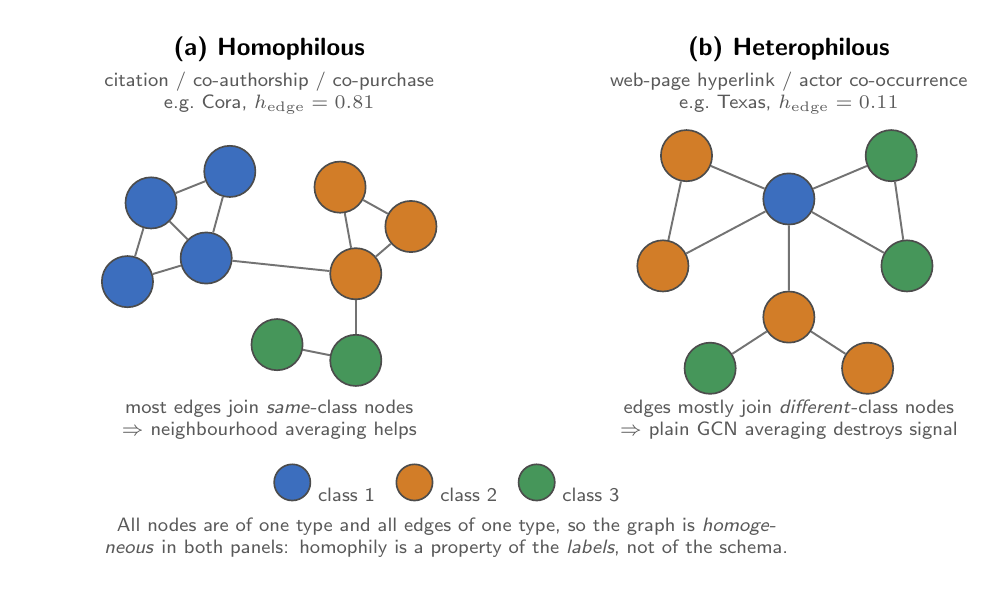
\begin{tikzpicture}[
  font=\small,
  v/.style={circle, draw=black!70, line width=0.6pt, minimum size=6.5mm,
            inner sep=0pt, font=\scriptsize\bfseries, text=white},
  e/.style={draw=black!55, line width=0.7pt},
  cut/.style={draw=red!75!black, line width=0.9pt, dash pattern=on 2pt off 1.6pt},
  ttl/.style={font=\small\bfseries, align=center},
  sub/.style={font=\scriptsize, align=center, text=black!65},
]

% ============ (a) homophilous: citation-like ============
\begin{scope}[xshift=0cm]
  \node[ttl] at (2.1,3.45) {(a) Homophilous};
  \node[sub] at (2.1,2.9) {citation / co-authorship / co-purchase\\
                           e.g.\ Cora, $h_{\mathrm{edge}}=0.81$};

  \node[v,fill=clsA] (a1) at (0.6,1.5) {};
  \node[v,fill=clsA] (a2) at (1.6,1.9) {};
  \node[v,fill=clsA] (a3) at (1.3,0.8) {};
  \node[v,fill=clsA] (a4) at (0.3,0.5) {};
  \node[v,fill=clsB] (b1) at (3.0,1.7) {};
  \node[v,fill=clsB] (b2) at (3.9,1.2) {};
  \node[v,fill=clsB] (b3) at (3.2,0.6) {};
  \node[v,fill=clsC] (c1) at (2.2,-0.3) {};
  \node[v,fill=clsC] (c2) at (3.2,-0.5) {};

  \draw[e] (a1)--(a2) (a1)--(a3) (a2)--(a3) (a3)--(a4) (a1)--(a4);
  \draw[e] (b1)--(b2) (b1)--(b3) (b2)--(b3);
  \draw[e] (c1)--(c2);
  % the few cross-class edges
  \draw[e] (a3)--(b3);
  \draw[e] (b3)--(c2);

  \node[sub] at (2.1,-1.25) {most edges join \emph{same}-class nodes\\
                             $\Rightarrow$ neighbourhood averaging helps};
\end{scope}

% ============ (b) heterophilous: web-page-like ============
\begin{scope}[xshift=6.6cm]
  \node[ttl] at (2.1,3.45) {(b) Heterophilous};
  \node[sub] at (2.1,2.9) {web-page hyperlink / actor co-occurrence\\
                           e.g.\ Texas, $h_{\mathrm{edge}}=0.11$};

  \node[v,fill=clsA] (h1) at (2.1,1.55) {};
  \node[v,fill=clsB] (h2) at (0.8,2.1) {};
  \node[v,fill=clsC] (h3) at (3.4,2.1) {};
  \node[v,fill=clsB] (h4) at (0.5,0.7) {};
  \node[v,fill=clsC] (h5) at (3.6,0.7) {};
  \node[v,fill=clsB] (h6) at (2.1,0.05) {};
  \node[v,fill=clsC] (h7) at (1.1,-0.6) {};
  \node[v,fill=clsB] (h8) at (3.1,-0.6) {};

  \draw[e] (h1)--(h2) (h1)--(h3) (h1)--(h4) (h1)--(h5) (h1)--(h6);
  \draw[e] (h6)--(h7) (h6)--(h8);
  \draw[e] (h2)--(h4) (h3)--(h5);

  \node[sub] at (2.1,-1.25) {edges mostly join \emph{different}-class nodes\\
                             $\Rightarrow$ plain GCN averaging destroys signal};
\end{scope}

% legend, centred under both panels and wrapped so the figure stays ~2:1
\node[sub] at (4.35,-2.05)
  {\tikz\node[v,fill=clsA,minimum size=4.6mm]{};\ class 1\quad
   \tikz\node[v,fill=clsB,minimum size=4.6mm]{};\ class 2\quad
   \tikz\node[v,fill=clsC,minimum size=4.6mm]{};\ class 3};
\node[sub, text width=10.4cm] at (4.35,-2.75)
  {All nodes are of one type and all edges of one type, so the graph is
   \emph{homogeneous} in both panels: homophily is a property of the
   \emph{labels}, not of the schema.};

\end{tikzpicture}
\end{document}
